\documentclass[10pt, a4paper]{jreport}

\usepackage[dvipdfmx]{graphicx}
\usepackage{here}
\usepackage{comment}
\usepackage{otf}
\usepackage{framed}

\usepackage{listings}
\renewcommand{\lstlistingname}{ソースコード}
%\usepackage{color}
\lstset{%
  %language={C},
  basicstyle={\small},%
  identifierstyle={\small},%
  commentstyle={\small\itshape\color[rgb]{0,0.5,0}},%
  keywordstyle={\small\bfseries\color[rgb]{0,0,1}},%
  ndkeywordstyle={\small},%
  stringstyle={\small\ttfamily\color[rgb]{1,0,1}},
  frame={tb},
  breaklines=true,
  columns=[l]{fullflexible},%
  numbers=left,%
  xrightmargin=0zw,%
  xleftmargin=3zw,%
  numberstyle={\scriptsize},%
  stepnumber=1,
  numbersep=1zw,%
  lineskip=-0.5ex%
}

% \title{タイトル}
% \author{}
% \date{}

\begin{document}
% \maketitle

% ----------------------------------------------------------------------------------------------------

\chapter{はじめに}
インターネットの急速な普及に伴って,情報のアクセスが容易になり,我々の生活が豊かになった一方で,インターネットを悪用したサイバー犯罪が横行している.

サイバー犯罪は,サーバやアプリケーションの脆弱性を利用して,アクセス権限を要する情報を不正に入手したり,サーバに莫大な負荷をかけて,サービスに支障をきたしたりする行為のことである.サイバー犯罪の被害として,顧客の個人情報が流出したり,サービスが長期間,利用できなくなることなどが挙げられる.これらの被害は,サービスを利用する顧客にとっても,サービスを運営する企業にとっても大きな損失となるため,サイバー犯罪の被害を未然に防ぐことはもちろん,被害に遭った際に犯人を特定するための対策を講じることも重要である.

サイバー犯罪の犯人を特定する情報として,多くの場合,IPアドレスが用いられる.サイバー犯罪の被害を受けたサーバのログから,サイバー犯罪に該当するアクセスのIPアドレスを捜査し,インターネットサービスプロバイダに照会を要請することで,犯人の身元を特定することができる.

しかし,技術の進歩により,近年では,IPアドレスのみによる個人の特定は困難になってきている.VPNやTorを用いることで,インターネットサービスプロバイダから割り振られている本来のIPアドレスを秘匿化してインターネットに接続することができる.また,キャリアグレードNATの普及により,通常よりIPアドレスでの個人の特定が難しくなっていることも事実である.これらの技術についての詳細は,次章で後述する.

そこで,本論文では,サイバー犯罪が発生した際に,IPアドレス以外の方法で犯人を特定する手法について提案する.インターネット利用者が,サーバに送信する情報は複数挙げられるが,その中でもCookieに着目した特定システムを提案する.Cookieは,WebサーバがWebブラウザに対して,任意の文字列を記憶させるための仕組みである.サーバからCookieを保存するように指示されたブラウザは,以降,そのWebサイトに対して,記憶したCookieを送信するようになる.

Cookieを利用することで,サービスのログイン状態を記憶したり,ECサイトにおいて,ショッピングカートの中身を記憶させたりすることができる.一方で,アクセスしてきたユーザに,ユニークな文字列を発行し,Cookieとして保存させることで,過去にそのユーザがアクセスしてきたかどうかがわかるため,個人を特定するために用いられることもある.このように,Cookieはユーザを特定する十分な情報となり得る.

% ここに,この論文の章立ての説明を書く.
\newpage
















%サイバー犯罪が起こった際に,IPアドレスなどで犯人を特定するが,最近では,キャリアグレードNATなどの技術の普及により,IPアドレスでの追跡は困難となっている.そこで,IPアドレス以外の情報,たとえばCookieなどを用いることで犯人を特定する手法について提案する.
\chapter{研究背景}
\section{IPアドレスによる特定の難しさ}
発信元のIPアドレスを特定することで,発信者の利用しているインターネットサービスプロバイダやキャリア,地域レベルの位置情報を取得できることが多い.サイバー犯罪が発生した際に,IPアドレスからインターネットサービスプロバイダを特定し,インターネットサービスプロバイダに照会を要請することで犯人を特定することができる.

しかし,技術の進歩により,IPアドレスによる個人の特定は困難であるケースも珍しくない.IPアドレスによる個人の特定が困難となる技術の代表例を以下に示す.

\subsection{キャリアグレードNAT}
キャリアグレードNATとは,インターネットサービスプロバイダなどが,ネットワークアドレス変換(NAT)を行う仕組みである.ネットワークアドレス変換とは,同一LAN内の各端末に割り振られたプライベートIPアドレスと,インターネットサービスプロバイダから割り振られたグローバルIPアドレスを変換するための仕組みである.IPv4アドレスの枯渇問題により,インターネットに接続する各端末すべてにグローバルIPアドレスを割り振ることは困難である.そこで,各端末には,グローバルIPアドレスの代わりに,プライベートIPアドレスを割り振り,インターネットに接続する際に,プライベートIPアドレスをグローバルIPアドレスに変換することで,LAN内の複数の端末を同じグローバルIPアドレスでインターネットに接続させることができる.ネットワークアドレス変換は,各家庭のLAN内で行われるが,これをインターネットサービスプロバイダ単位で行ったものがキャリアグレードNATである.

IPv4アドレスの枯渇問題を解消する手段として,キャリアグレードNATがしばしば利用されているが,同一のグローバルIPアドレスが,複数のインターネット利用者によって使用されるため,キャリアグレードNATを使用している場合は,IPアドレスによる個人の特定が困難となる.インターネットサービスプロバイダでは,キャリアグレードNATを利用した際のIPアドレスの変換テーブルを保持しているが,変換テーブルは,最新の約2ヶ月分しか記録されていないため,保存期間を過ぎると,IPアドレスによる特定ができなくなる.

\subsection{VPN}

\subsection{Tor}

\section{IPアドレスによる誤認逮捕}

\section{Cookieによる個人の特定}
IPアドレスによる個人の特定は困難であったり,誤認逮捕を招く可能性があるため,サイバー犯罪において犯人を特定する情報としては,十分とはいえない.そこで,本論文では,Cookieによる個人の特定可能性に着目した.

Cookieとは,Webサーバが,Webブラウザに対して,任意の情報(文字列)を記憶させるための仕組みである.サーバからCookieを保存するように指示されたブラウザは,以降,そのWebサイトに対して,記憶したCookieを送信するようになる.

Cookieを利用することで,サービスのログイン状態を記憶したり,ECサイトにおいて,ショッピングカートの中身を記憶させたりすることができる.一方で,アクセスしてきたユーザに,ユニークな文字列を発行し,Cookieとして保存させることで,過去にそのユーザがアクセスしてきたかどうかを調べることができる.このように,Cookieはユーザを特定する十分な情報となり得る.

ブラウザがサーバに送信する情報として,使用している言語,ブラウザやOSの種類,バージョンなどが挙げられるが,これらは他のユーザと似たような情報となることが多い上,本来とは異なる情報を送信することも可能である.それに対して,Cookieは,サーバがブラウザに保存するように指示する値であるため,サーバがユニークな値を発行し,発行した値を記録しておくことができる.そのため,他のユーザと区別することができる上,ユーザが,サーバから指示された値とは異なるCookieを送信しても,詐称したことがわかる.よって,Cookieは,ブラウザがサーバに送信する情報の中でも,個人を特定できる可能性が高いことがわかる.

\section{SNSによる個人の特定}
%参考文献に出典をまとめる!
近年,多くのインターネット利用者がSNSを利用している.Twitter社が公開した"Q2 2017 Letter to Shareholders"によれば,2017年におけるTwitterの月間利用者数は3億2800万人である.また,Facebook社が公開した"Facebook Q2 2017 Results"によれば,2017年におけるFacebookの月間利用者数は約20億人である.SNSが発展した現代においては,世界中の人々が,SNSを通じてインターネットに自分の情報を発信しているといえる.

TwitterやFacebookなどのSNSには,多くの個人情報が保存されている.そのため,サイバー犯罪の犯人が利用しているSNSのアカウントを特定し,SNSを運営する企業に協力を依頼することで,犯人の身元を特定することは十分に可能であると考えられる.

最近の多くのWebサイト,とりわけニュースサイトやブログサイトでは,自身もしくは自社のサイトを読者に広めてもらうために,SNSのシェアボタンを設置していることが多い.SNSのシェアボタンのリソース(画像やスクリプトなど)を読み込むために,ブラウザはSNSのサイトに対してリクエストを送信するが,その際に,ユーザがそのSNSにログインした状態であれば,SNSのサーバにセッション情報を含むCookieを送信しているはずである.

したがって,SNSのシェアボタンを設置したサイトでサイバー犯罪が発生した際,犯人がそのSNSにログインした状態であれば,犯人のSNSのアカウントを特定することができる可能性が高いと考えられる.Cookieが個人を特定する情報となり得ることについては前述したが,SNSのCookieはサイバー犯罪の犯人を特定する上で非常に重要な情報であるといえる.

\section{犯人の不注意による逮捕事例}
SNSによる特定は,犯人がSNSにログインしていることが前提である.用心深い犯人であれば,サイバー犯罪を行う前にSNSからログアウトしているか,別のブラウザを使用しているであろう.

%出典を明記したい。書かれていることが曖昧な可能性がある
しかし,すべてのサイバー犯罪の犯人が,完全に証拠を残さずに犯罪を行うわけではない.実際に,Torを利用して児童ポルノを投稿した犯人が逮捕された事例がある.Torを使用することで発信元を隠蔽することができるが,逮捕された犯人は,Torの利用中に,不注意により通常のブラウザを使用したために発信元を特定されてしまった.このように,犯人の不注意によって逮捕されるケースもある.

SNSにおいて,利用を中断する度にログアウトするユーザは少数であると考えられる.ログインした状態でも通常のインターネットの使用に支障がないためである.よって,SNSにログインした状態で,そのSNSのシェアボタンが設置されたサイトにアクセスすることは十分に考えられる.犯人の不注意によりSNSのアカウントを特定することは,犯人の特定に大きく寄与するといえる.

\newpage
















\chapter{研究方法}
\section{研究目的}
%第2章で書いたことをまとめる。こんな感じで
\begin{comment}
IPアドレスによる特定は難しい。誤認逮捕などもあるため問題である
↓
Cookieは個人を特定する上で重要な情報となり得る
↓
近年ではSNSが普及したことにより多くのユーザがSNSを利用するようになった
SNSは通常ログインしっぱなしであり、ログアウトすることはめったにない
↓
犯人がサイバー犯罪を行う際に、うっかりSNSにログインしたままである可能性がある
実際に、過去にはTorからサイバー犯罪を行った犯人が、うっかりふつうのブラウザを使ってしまったことで特定されてしまった
↓
SNSのシェアボタンに送信されたCookieを追跡することで、掲示板に書き込んだユーザを特定することができるのではないか
\end{comment}
第2章で述べたように,IPアドレスによる特定は困難である.そのため,サイバー犯罪の犯人を特定する際は,IPアドレスだけでなく,それ以外の情報を元に特定する手法が必要である.本論文では,Cookieが個人を特定できる可能性が高いことに着目した.また,近年においてSNSを利用するユーザが多く存在し,ログアウトする機会が少ないことから,サイバー犯罪において,犯人のSNSのアカウントを発見することが,犯人の特定に大きく寄与するのではないかと考えられる.最近では,SNSのシェアボタンを設置するWebサイトが多く見受けられる.SNSのシェアボタンを読み込む際に送信されたCookieを利用することで,サイバー犯罪の犯人を特定する手法を提案することを目的とする.

\section{提案手法}
SNSのシェアボタンを読み込む際に送信されたCookieから,個人をどの程度特定できるか実験するために,本研究では,匿名掲示板サイトとSNSサイトを用意した.

\newpage










\chapter{実装}
\section{匿名掲示板}
本研究で使用した匿名掲示板は,インターネット上にフリーソフトウェアとして公開されているKENT-WEBのLIGHT BOARD(以下,LIGHT BOARD)である.この掲示板は,アカウント登録が不要で利用できる掲示板サイトである.名前の入力が必須となっているが,実名を入力する必要はなく,投稿毎に別の名前を入力することも可能であるため,匿名掲示板として利用することができる.

本研究では,LIGHT BOARDのソースプログラムをダウンロードし,改変したものを,自身のサーバで公開し実験を行った.実験で使用した匿名掲示板サイトを図\ref{fig: bbs_screenshot}に示す.

\begin{figure}[H]
	\begin{center}
		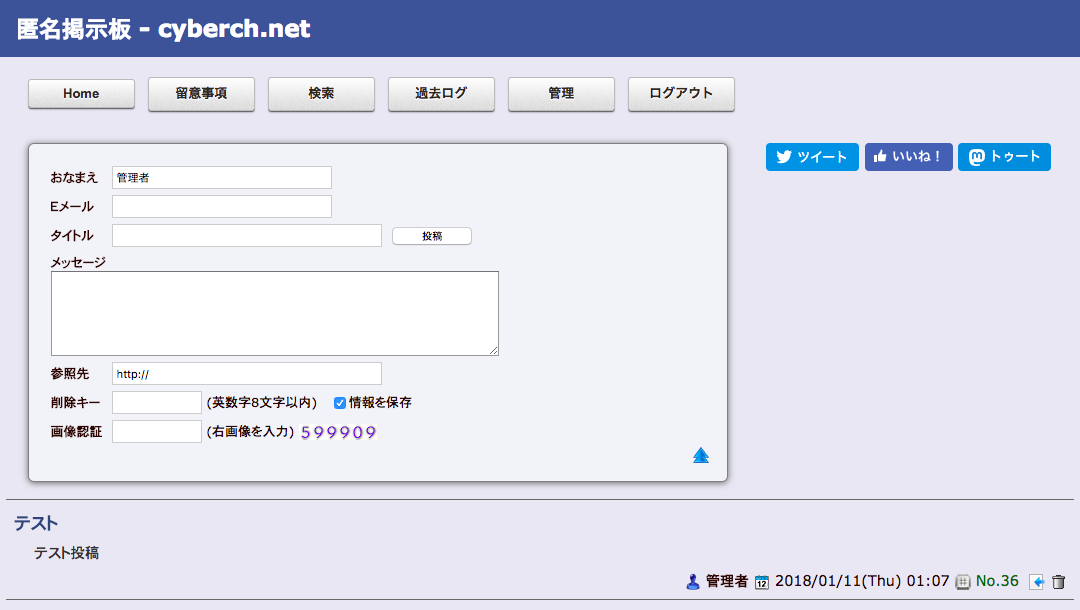
\includegraphics[width=130mm]{figures/bbs_screenshot.png}
	\end{center}
	\caption{匿名掲示板サイト}
	\label{fig: bbs_screenshot}
\end{figure}

掲示板への書込みの際に入力する項目は複数あるが,必須項目は書込みを行った人の名前,書込みのタイトル,本文,画像認証の4項目である.画像認証の項目には,入力欄の右側に画像として表示された数字を入力する.これはスパム投稿を防止するためのものである.先述の通り,名前は実名を入力する必要はないため,個人情報を一切入力せずに投稿できるため,利用者から見ると匿名掲示板のように利用することができる.必須項目を入力して投稿ボタンを押下すると投稿内容がサーバに送信され,書込み一覧に投稿内容が表示される.

\subsection{シェアボタンの設置}
LIGHT BOARDにはシェアボタンは設置されていない.本研究では,SNSのシェアボタンを利用して実験を行うため,シェアボタンを設置した.設置したSNSのシェアボタンは,Twitter,Facebook,Mastodonの3種類である.

Mastodonのシステムは,匿名掲示板サイトと同様に,本研究の実験用に用意したサーバ上に置かれている.そのため,Mastodonのシェアボタンを読み込む際に送信されたCookieは,保存,解析することができる.送信されたCookieを保存し,そのCookieからMastodonのユーザを特定するプログラムを作成した.詳細は後述する.

\subsection{同一ユーザ特定機能の実装}
LIGHT BOARDは,書込み時に名前の入力が必須であるが,同一ユーザが複数の書込みを行う際に,それぞれ異なる名前をつけることが可能である.そのため,複数の書込みが同一人物によるものかどうかを判断することは難しい.そこで,本研究の実験で使用する匿名掲示板には,ユーザを追跡するためのCookieを付与する機能を実装した.

初めて匿名掲示板にアクセスしてきたユーザには,サーバ側で生成したランダムな文字列をCookieとして付与する.2回目以降にアクセスしてきたユーザ(ブラウザ)は,初めてアクセスした際に付与されたCookieをサーバに送信するため,以前にアクセスしたことがあることがサーバ側でわかる.したがって,複数の書込みを行ったユーザは,書込みを行う際に送信しているCookieが同じであるため,同一人物による書込みであることがわかる.

ユーザを追跡するためのCookieを付与する機能に該当する箇所をソースコード\ref{track}に示す.

\begin{lstlisting}[caption=同一ユーザ特定機能,label=track]
use String::Random;

sub track {
  my $host = $ENV{REMOTE_HOST};
  my $addr = $ENV{REMOTE_ADDR};
  my $time = time;
  my ($min,$hour,$mday,$mon,$year,$wday) = (localtime($time))[1..6];
  my @wk = ('Sun','Mon','Tue','Wed','Thu','Fri','Sat');
  my $date = sprintf("%04d/%02d/%02d(%s) %02d:%02d",
        $year+1900,$mon+1,$mday,$wk[$wday],$hour,$min);
  my $cookie = $ENV{HTTP_COOKIE};

  my %cookie;
  foreach (split(/;/, $cookie)) {
    my ($key, $val) = split(/=/);
    $key =~ s/\s//g;
    $cookie{$key} = $val;
  }

  # もしトラッキング用のクッキーがセットされていればファイルに保存する
  # 保存されていなければ新しく発行してセットさせる
  if ($cookie{tracking_id}) {
    open(DAT, ">> $cf{trackingfile}") or error("open err: $cf{trackingfile}");
    my $new = "$date<>$cookie{tracking_id}<>$host<>$addr";
    print DAT "$new\n";
    close(DAT);
  }
  else {
    my $random = String::Random->new();
    my $tracking_id = $random->randregex("[a-zA-Z0-9]{64}");
    print "Set-Cookie: $cf{tracking_id}=$tracking_id\n";
  }
}
\end{lstlisting}

サブルーチンtrackは,トラッキング(特定)用のCookieが送信されなければ新たにCookieを発行し,送信されていればそのCookieをファイルに保存する.発行するCookieは,String::Randomを使用して生成した乱数を値とする.String::Randomを使用して生成する乱数は,大文字,小文字を区別した64文字の英数字であるため,他のユーザと重複する可能性は極めて低いと考えられる.よって,匿名掲示板への書込みとトラッキング用のCookieを照らし合わせ,複数の書込みに対して同じCookieが送信されている場合,同一人物による書込みであると判断できる.

\section{SNS}
本研究では,SNSのアカウントを特定する実験を行うためのシステムとして,Mastodonを利用した.本来のサイバー犯罪においては,TwitterやFacebookなどの,世界的に利用されているSNSの運営と協力して犯人のアカウントを特定することを想定しているが,本研究の実験では,TwitterやFacebookのサーバ内の情報を閲覧することはできない.そこで,個人で運営することができる,Twitterに似たSNSであるMastodonを利用することで,シェアボタンを読み込む際に送信されるCookieからMastodonのアカウントを特定する実験を行った.送信されるCookieからアカウントを特定することは,TwitterやFacebookにおいても技術的に可能であるため,実際のサイバー犯罪ではTwitterやFacebookなどの運営と協力することで,犯人のアカウントが特定できるといえる.

\subsection*{Mastodon}
Mastodonとは,ドイツ人のEugen Rochko氏が,2016年2月に開発を開始した,分散型SNSのことである.Twitterに似た機能を持つSNSとして日本でも注目を集めている.オープンソースソフトウェアとしてGitHub上に公開されており,誰でも自由にプログラムを利用することができる.

TwitterやFacebookとは異なり,Mastodonはプログラムを改変することができ,また改変したプログラムをサーバ上に置いて運営することもできる.GitHubからダウンロードしたMastodonのプログラムに,本研究の実験に必要な機能を実装して利用した.

\subsection{シェアボタンの実装}
匿名掲示板に設置するシェアボタンの実装を行った./buttonというURLにアクセスすると,Mastodonのシェアボタンの画像だけが表示されるページを作成した.匿名掲示板では,HTMLのiframeタグを利用し,Mastodonのシェアボタンのページを読み込んでいる.

ユーザ(ブラウザ)は,匿名掲示板にアクセスした際に,Mastodonのシェアボタンを読み込むためにMastodonのサーバにアクセスする.Mastodonのサーバにアクセスする際に,もしユーザがMastodonにログインしている状態であれば,そのログイン状態を保持するCookieをMastodonのサーバに送信するため,匿名掲示板にアクセスしたユーザとMastodonにログインしているユーザを結びつけることができる.

\subsection{送信されたCookieを保存する機能の実装}
匿名掲示板に設置されたシェアボタンを通してMastodonのサーバに送信されたCookieをデータベースに保存する機能を実装した.Mastodonのシェアボタンが読み込まれた際に,送信元の情報を取得し,データベースに保存している.保存する送信元の情報を表\ref{tb: buttons_database}に示す.

\begin{table}[H]
	\caption{保存した送信元のデータ}
	\label{tb: buttons_database}
	\begin{center}
		\begin{tabular}{ | c | c | p{8cm} | } \hline
			データ & データ型 & データ例 \\ \hline
			IPアドレス & string & 133.19.169.6 \\ \hline
			Cookie & text & remember\_user\_token=ABCD1234; \_session\_id=EFGH5678; \_mastodon\_session=IJKL9012  \\ \hline
			リファラ & string & https://www.google.co.jp/ \\ \hline
			ユーザエージェント & string &  Mozilla/5.0 (Macintosh; Intel Mac OS X 10\_12\_6) AppleWebKit/537.36 (KHTML, like Gecko) Chrome/62.0.3202.94 Safari/537.36 \\ \hline
		\end{tabular}
	\end{center}
\end{table}

取得したデータは,IPアドレス,Cookie,リファラ,ユーザエージェントの4つである.データ型は,データベースに保存する際の型を意味する.データ例は,実際に保存されるデータの例を示している.

データベースには,Cookieの他に送信元のIPアドレスやリファラ,ユーザエージェントを保存している.本研究においてはCookieのみの保存で十分であるが,Cookieが取得できなかった場合や,より詳細な情報を得るために,Cookie以外の情報も保存することにした.

\subsection*{リファラ}
リファラとは,どのページからアクセスしたかを示す情報である.例えば,Googleの検索結果からリンクをクリックしてサイトAにアクセスした場合,ブラウザがサイトAに対して送信するリファラはhttps://www.google.co.jp/である.リンクをクリックしてページを遷移した場合に限らず,iframeを使用して別のサイトを読み込んだ場合にもリファラは送信される.匿名掲示板のHTML内に含まれるiframeタグからMastodonのページを読み込んだ場合,Mastodonのサーバに送信されるリファラは,匿名掲示板のURLである.このように,リファラはどのページを経由してアクセスしてきたかがサーバ側にわかるため,Webサイトの解析ツールなどでしばしば用いられる.

\subsection*{ユーザエージェント}
ユーザエージェントとは,ブラウザがサーバに対して送信する情報であり,使用しているブラウザやOS,またその種類などの情報が含まれている.例えば表\ref{tb: buttons_database}のデータ例の場合,アクセスしてきたユーザは,macOS 10.12.6を使用しており,Google Chrome 62.0.3202.94でアクセスしていることがわかる.使用しているブラウザごとにWebページの表示を変えるなど,ユーザビリティの向上を目的に使用されることもあるが,サイバー犯罪においては,犯人の使用しているOSやブラウザがわかるといった利点がある.ただし,ユーザエージェントは詐称(本来とは異なる情報をサーバ側に送信)することも可能であるため,必ずしもユーザエージェントと同じOSやブラウザを使用しているとは限らない.









































\begin{comment}
表の挿入はここから
\begin{table}[H]
	\caption{表のタイトルを入力}
	\label{tb: example1}
	\begin{center}
		\begin{tabular}{ | c | c | c | } \hline
			タイトル & タイトル & タイトル \\ \hline\hline
			内容1-1 & 内容1-2 & 内容1-3 \\ \hline
			内容2-1 & 内容2-2 & 内容2-3 \\ \hline
		\end{tabular}
	\end{center}
\end{table}
表の挿入はここまで
表\ref{tb: example1}のように表番号を参照することができます.
\end{comment}

\begin{comment}
図の挿入はここから
\begin{figure}[H]
	\begin{center}
		\includegraphics[width=(好きな数値)mm]{画像ファイル名を入力}
	\end{center}
	\caption{図のタイトルを入力}
	\label{fig: example1}
\end{figure}
図の挿入はここまで
図\ref{fig: example1}のように図番号を参照することができます.
\end{comment}





\end{document}